% This version of CVPR template is provided by Ming-Ming Cheng.
% Please leave an issue if you found a bug:
% https://github.com/MCG-NKU/CVPR_Template.

\documentclass[review]{cvpr}
%\documentclass[final]{cvpr}

\usepackage{times}
\usepackage{epsfig}
\usepackage{graphicx}
\usepackage{amsmath}
\usepackage{amssymb}
\usepackage{bbm}
% Include other packages here, before hyperref.

\usepackage{array}
\usepackage{multirow}
\usepackage{longtable}
\usepackage{tabularx}
%\usepackage{subfigure}
\usepackage{algorithm}
\usepackage{algorithmicx}
\usepackage{algpseudocode}
\usepackage{arydshln}
\usepackage{pifont}% http://ctan.org/pkg/pifont
\usepackage{url}
\usepackage{booktabs}
%\numberwithin{figure}{document}
\newcommand{\cmark}{\ding{51}}%
\newcommand{\xmark}{\ding{55}}%
\algnewcommand\algorithmicinput{\textbf{Input:}}
\algnewcommand\INPUT{\item[\algorithmicinput]}
\algnewcommand\algorithmicoutput{\textbf{Output:}}
\algnewcommand\OUTPUT{\item[\algorithmicoutput]}
\def\BB{\textcolor{blue}}
\def\RR{\textcolor{black}}
\DeclareMathOperator*{\argmax}{arg\,max}
\DeclareMathOperator*{\argmin}{arg\,min}
\global\long\def\defeq{\stackrel{\mathrm{{\scriptscriptstyle def}}}{=}}




\global\long\def\otilde{\widetilde{O}}
% If you comment hyperref and then uncomment it, you should delete
% egpaper.aux before re-running latex.  (Or just hit 'q' on the first latex
% run, let it finish, and you should be clear).
\usepackage[pagebackref=true,breaklinks=true,colorlinks,bookmarks=false]{hyperref}


\def\cvprPaperID{2672} % *** Enter the CVPR Paper ID here
\def\confYear{CVPR 2021}
%\setcounter{page}{4321} % For final version only


\begin{document}

%%%%%%%%% TITLE
\title{MaskSparsity: Pruning the Convolutional Neural Networks via Fine-Grained Sparse Regularization}

\author{First Author\\
Institution1\\
Institution1 address\\
{\tt\small firstauthor@i1.org}
% For a paper whose authors are all at the same institution,
% omit the following lines up until the closing ``}''.
% Additional authors and addresses can be added with ``\and'',
% just like the second author.
% To save space, use either the email address or home page, not both
\and
Second Author\\
Institution2\\
First line of institution2 address\\
{\tt\small secondauthor@i2.org}
}

\maketitle


%%%%%%%%% ABSTRACT
\begin{abstract}
 

Structural neural network pruning aims to remove the redundant channels in the deep convolutional neural networks (CNNs) by pruning the filters of less importance to the final output accuracy. To reduce the degradation of performance after pruning, many methods utilize sparse regularization loss to produce structured sparsity. In this paper, we analyze these sparsity-training-based methods and find out two problems of these methods. First, the regularization of unpruned channels is unnecessary, which also restricts the network's capacity. Second, the distribution of important filters and unimportant filters are not well distinguishable after sparsity-training. This challenges the selecting of pruning threshold. The consequence is that a part of pruned parameters are still not small enough to reduce the effect of pruning on the network's output. To solve this problem, we propose a novel pruning method with fine-grained sparse regularization, named MaskSparsity.  MaskSparsity imposes the sparse regularization on the specific filters selected by a predefined mask, rather than all the filters of the model. There are many ways to get the mask acquisition. In this paper, we use the pruning mask of the NetSlim method \cite{liu2017learning}. MaskSparsity achieves 58.2\%-FLOPs reduction on ResNet-110 by removing 59.2\% of the parameters, with only a small loss of 0.14\% in top-1 accuracy on CIFAR-10. Moreover, on ILSVRC-2012, MaskSparsity reduces more than 42\% FLOPs on ResNet-101 by removing 59.2\% of the parameters, with only a loss of 1.17\% in the top-1 accuracy.

\begin{figure}[h!]
	\begin{centering}
	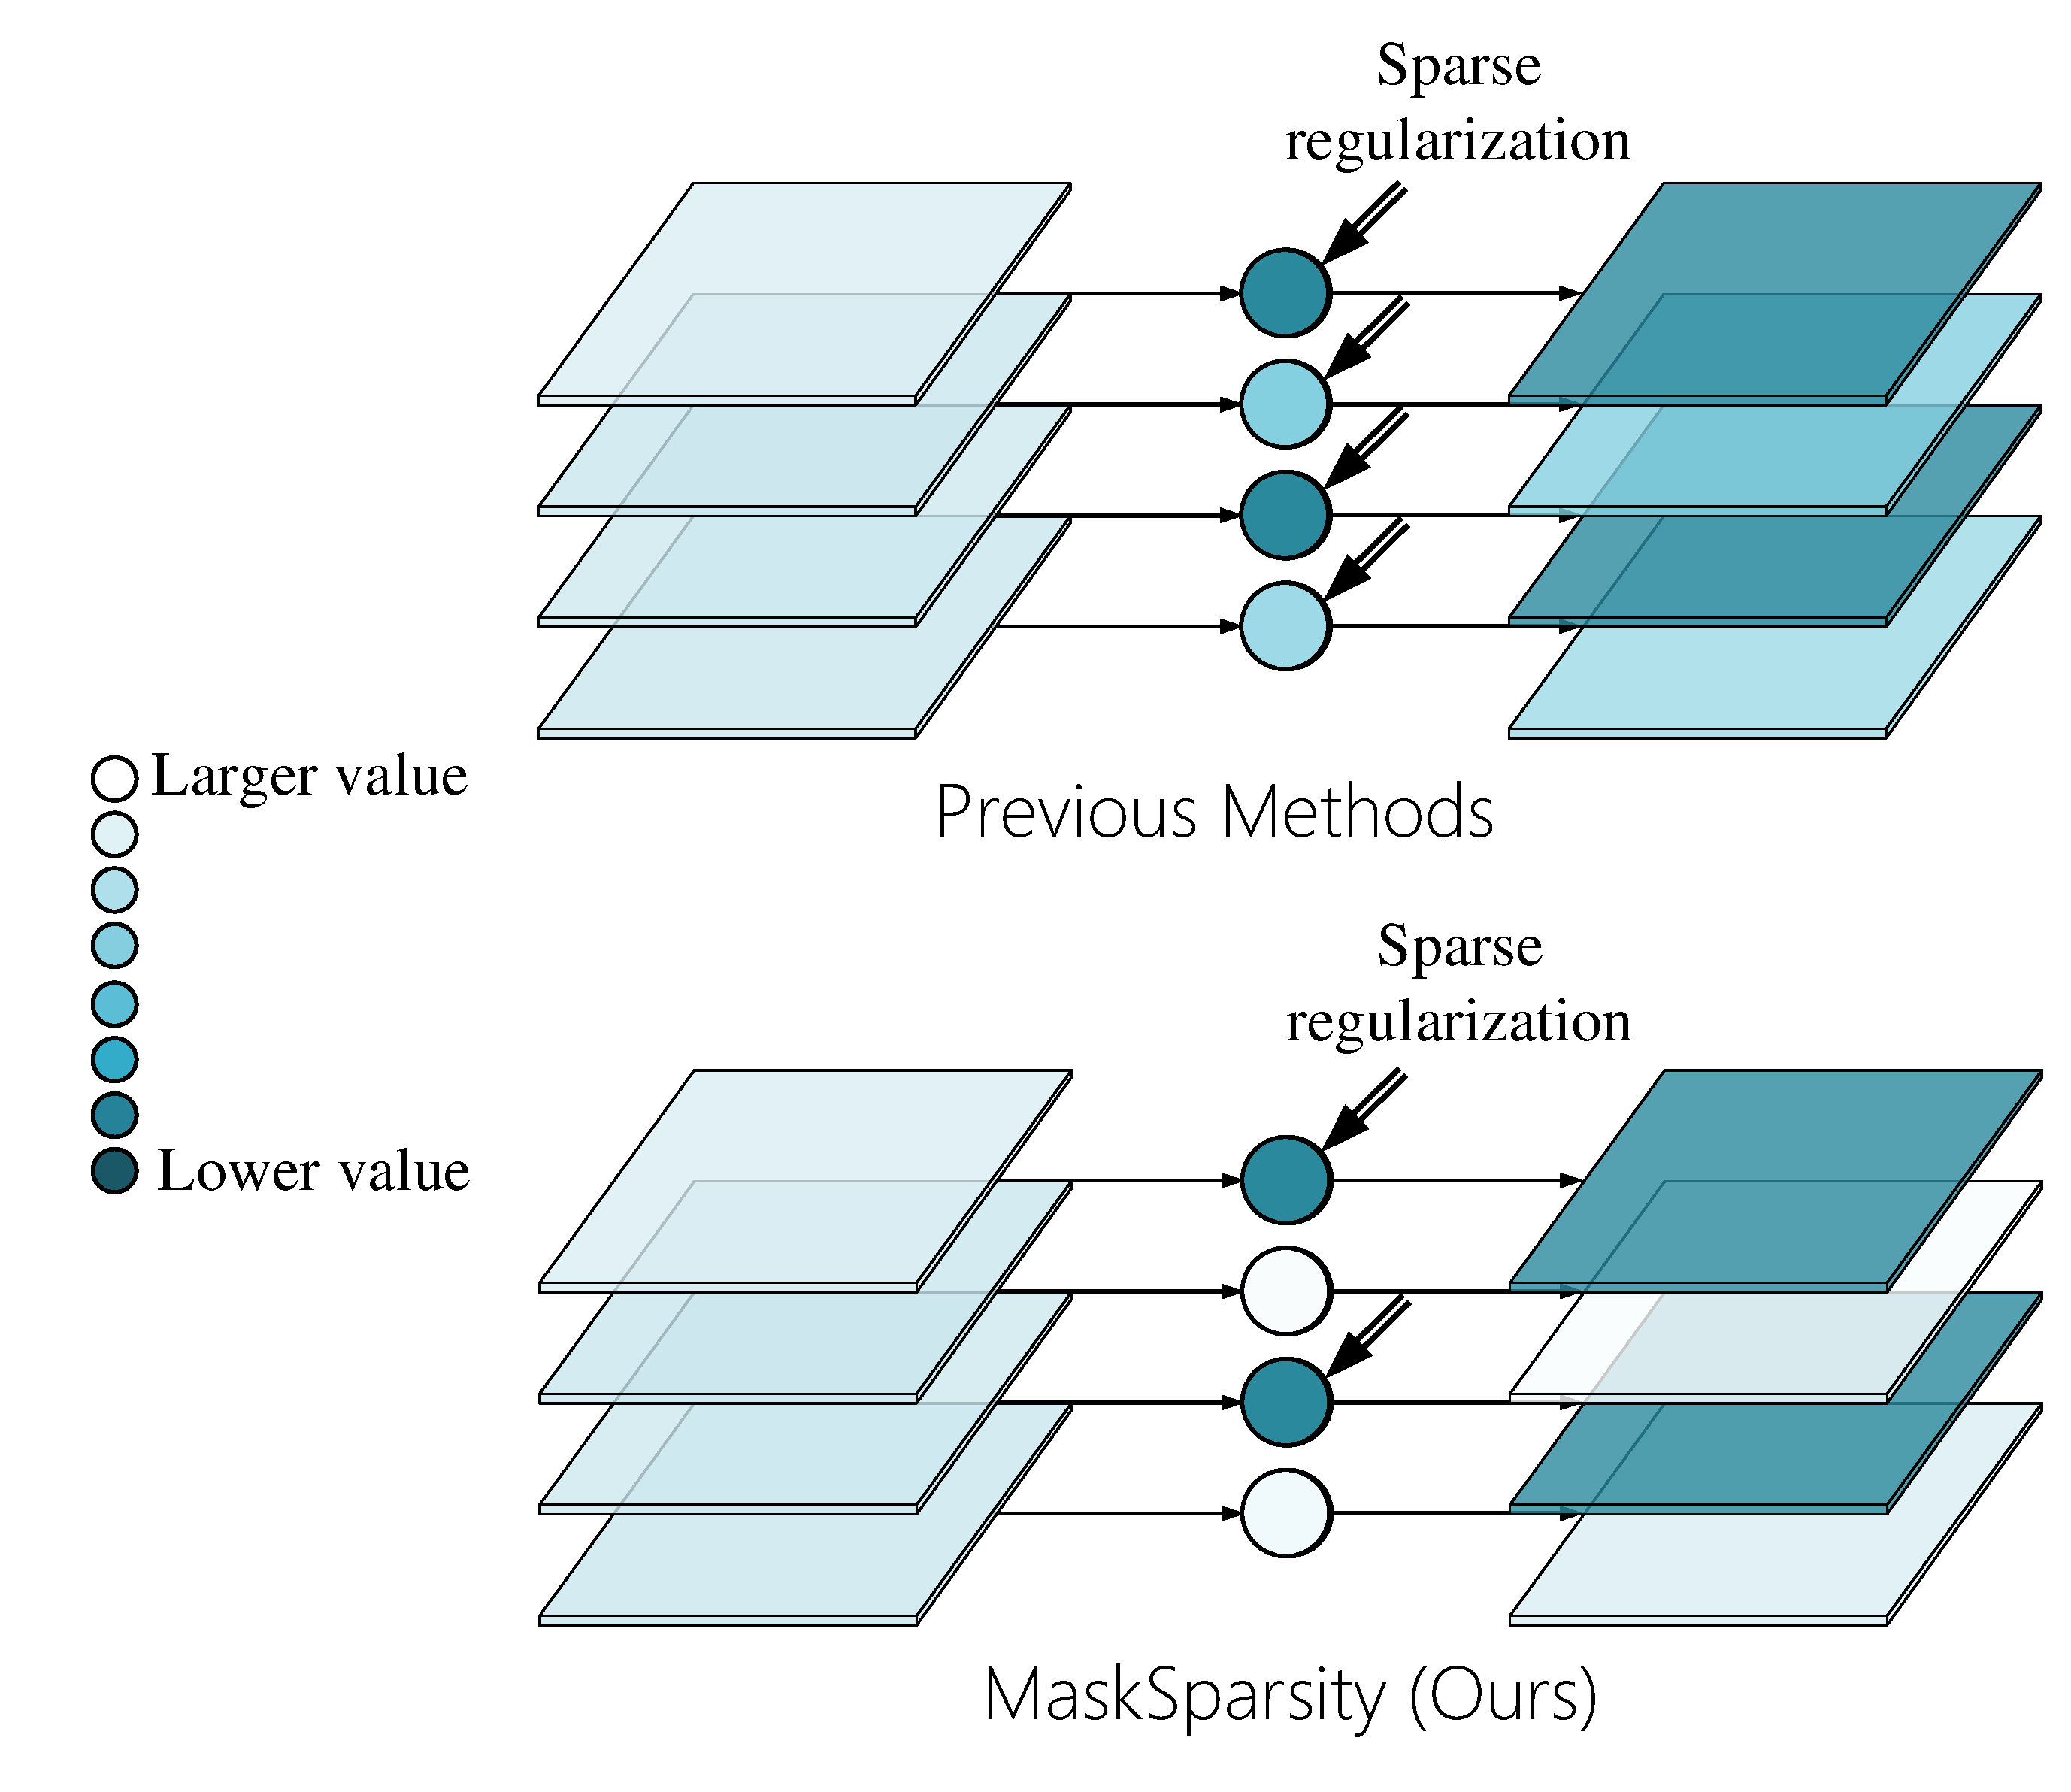
\includegraphics[width=0.95\linewidth]{figure/Masksparsity_v1.pdf}
	\caption{Visual comparison between the previous sparsity-training-based methods and the proposed MaskSparsity method.}
	\label{MAskSparsit}
	\par\end{centering}	
\end{figure}





 
\end{abstract}

%%%%%%%%% BODY TEXT
\section{Introduction}\label{introduction}

\begin{figure*}[]
	\centering
	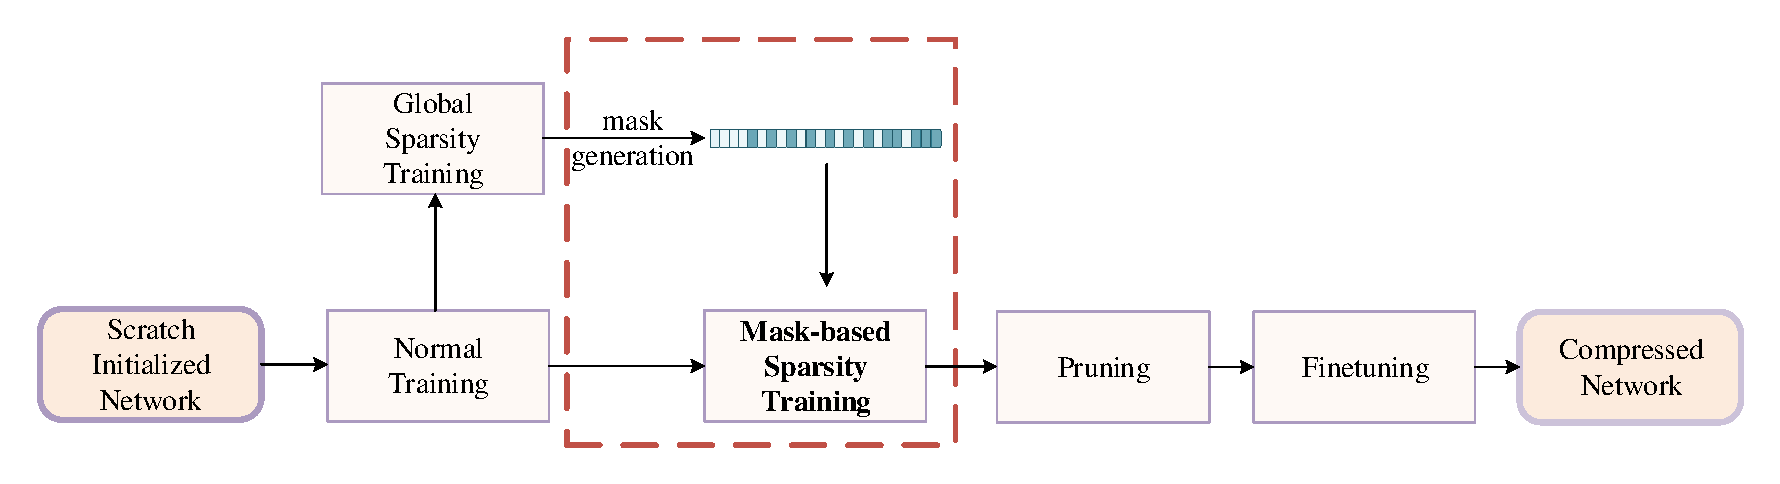
\includegraphics[width=0.95\linewidth]{figure/MaskSparsity.pdf}
	\vskip -0.1in
	\caption{The pipeline of the proposed MaskSparsity method.}
	\label{MAskSparsityPipeline}
	\vskip -0.15in
\end{figure*}


Convolutional Neural Networks (CNNs) have demonstrated a great success for a variety of computer vision tasks, like image classification \cite{russakovsky2015imagenet}, detection \cite{lin2014microsoft}, and semantic segmentation \cite{Cordts2016Cityscapes}.  However, the increasing depth and width of the CNNs also leads to the higher computing resources demands and excessive memory footprint requirements. Typically, the widely used ResNet models \cite{he2016deep} have millions of parameters, requiring billions of float point operations (FLOPs), which makes it a great challenge to deploy most state-of-the-art CNNs on edge devices. As recent studies have reveal existence of the significant redundancy in deep CNNs \cite{denil2013predicting}, various methods were proposed to compress and accelerate CNNs, including network pruning \cite{li2020group}, parameter quantization \cite{jacob2018quantization}, knowledge distillation \cite{hinton2015distilling} and low-rank decomposition \cite{denton2014exploiting}. Network pruning is attracting much attention from the researchers. It removes the parameters in the deep CNNs and reduces the required FLOPs and memory footprint.

Existing network pruning methods can be divided into non-structural and structural pruning methods, according to the difference in the pruning granularity. Non-structural pruning methods delete the unimportant connections in the filter. They would result in irregular network structures, which is not supported on most deep learning libraries and devices. This limits the acceleration and applications of pruned network on general-purpose hardware. Structural pruning removes the whole filters of less importance according to a certain criterion. The pruned structure still consists of regular convolution layers. Therefore, this category of methods are more implementation-friendly, and they have more practical values. 

A typical scheme of network pruning consists of three stages: 1) training an over-parameterized model normally; 2) pruning the model according to a certain criterion; and 3) fine-tune the pruned model to reduce the degradation caused by pruning. Some of the existing network pruning methods apply a sparsity training stage after the Step 1). These methods apply sparse regularization on the filter weights of the convolution layers \cite{alvarez2016learning,wen2016learning} or scaling factors \cite{huang2018data,liu2017learning} of the batch normalization layers. After the sparsity training, the corresponding filter weights or scaling factors of unimportant channels are considered to be near 0. Then these channels could be safely pruned without affecting the output values of the corresponding layers too much. We call these methods as sparsity-training-based methods. 
 
However, we find that existing sparsity-training-based methods have the following two problems. First, the important channels are preserved after the pruning. However, the weights of these channels are still regularized in the sparsity training stage. We think this prevents the better coverage of the network in the sparsity training stage, which affects the final performance of the fine-tuned pruned network. Second, we find in the existing sparsity-training-based methods, the bad distribution of parameters after sparsity-training challenges the selecting of pruning threshold. The consequence is that a part of pruned parameters are still not small enough to be pruned without affecting the output of the network. In other words, these methods are not able to make the filter weights of these unimportant channels coverage to 0. In other words, these methods are not able to make the filter weights of these unimportant channels coverage to 0. We find this is cause by the full regularization on all channels of each layer, which leads to a lager gradients from the loss function for these unimportant layers. The gradients prevents the filter weight from decaying to 0 by the sparse regularization.


To address the problems mentioned above, we propose a novel sparsity-training-based channel pruning approach, named MaskSparsity. Different from the previous sparsity-training-based methods which with impose regularization on all channels of each layer of the network, MaskSparsity only imposes regularization on the specific channels selected by mask indicating the unimportant channels. In other words, we will only impose regularization on the channels to be pruned, and only prune the channels where regularization is applied. The perfect match between the sparse channels and the pruning channels allows us to minimizes the impact of sparse regularization and maximize the accuracy of the pruned networks, which solves the first problem above. With the the MaskSparsity method, the sparse training is able to push the filter weights of unimportant channels to a nearer-to-zero value, which makes the pruning threshold better to be set.

To summarize, our main contributions are three-fold:

(1)	We analyze the previous sparsity-training-based methods in the previous work, which simply impose L1 regularization on all channels of model. We elaborate on many of its problems.

(2)	We propose MaskSparsity to solve these problems by more fine-grained sparsity-training.

(3)	The extensive experiments on two benchmarks demonstrates the effectiveness and efficiency of MaskSparsity.



\section{Related Work}
We mainly focus on the structural pruning methods in this paper.
In this section, we first review the closely related works, \ie the sparsity-training-based structural pruning methods. After that, we list other structural pruning methods.

\subsection{Sparsity-training-based Pruning Methods}
To make the network adaptively converge to a sparse structure and alleviate the damage of the pruning process to the network's output, some sparsity-training-based pruning methods are prosed. There are mainly two categories of these methods according to the place where sparse regularization is applied. 

The first category of methods are the group sparsity based methods which apply the spare regularizations on the filter weights. Alvarez and Salzmann \cite{alvarez2016learning} proposed to use group sparsity regularizer to determine the number of channels of each layer. Wen \etal \cite{wen2016learning} proposed a Structured Sparsity Learning (SSL) method to regularize the structure to obtain a hardware-friendly pruned structure.  Alvarez and Salzmann \cite{alvarez2017compression} added a low-rank regularizer to improve the pruning performance. Zhang \etal proposed a group ordered weighted L1 regularizer. Li and Qi \cite{OICSROS} pointed out the correlations between two consecutive layers and proposed to combine one out-channel in current layer and the corresponding inchannel in next layer as a regularization group. Li and Gu proposed the Hinge \cite{Hinge} by combining the filter pruning and low-rank decomposition into the group sparsity training framework.

 
The second category of methods are the indirect group-sparse methods, which apply the sparse regularization on the scaling factors of each layer. The representative method is NetSlim \cite{liu2017learning} method, which sparsely regularizes the scaling factors of BN layers to get the sparse structure and remove less important channels. Huang and Wang \cite{huang2018data} proposed to add a new scaling factor vector to each layer to apply the sparse regularization. Srinivas and Subramanya \cite{Srinivas2017TrainingSN} proposed to impose sparse constraint over each weight with additional gate variables, and achieve high compression rates by pruning connections with zero gate values. Ye and You \cite{OT} proposed to to prune channels with layer dependent thresholds according to the different weight distribution of each layer. \cite{Dependency} develop the norm-based importance estimation by taking the dependency between the adjacent layers into consideration.
 

These methods all apply the global sparse regularization on the network channels, which over-regularize the important channels. Our MaskSparsity method solves this problem and is able to improve the performance of sparsity-training-based methods to the new state-of-the-art.

\subsection{Non-sparsity-training-based Pruning Methods}
Recently, many non-sparsity-training-based pruning methods also show good  performance. These methods usually evaluate the importance of each channels with a handcraft criterion first. After that, they directly prune the unimportant channels and finetune the network.
For instance, Li and Kadav \cite{L1} propose to prune filters with smaller L1 norm values in a network. Base on the theory of Geometric Median (GM) \cite{GM}, He and Liu proposed FPGM\cite{FPGM} to prune the filters with the most replaceable contribution. Inspired by the discovery that the average rank of multiple feature maps generated by a single filter is always the same, Lin et al \cite{lin2020hrank} propose to prune filters by exploring the High Rank of feature maps (HRank).  
In this paper, we compare the performance of the proposed MaskSparsity with these methods, and shows the good pruning performance.

 


\section{Methodology}

\subsection{Notations and background}\label{Notations-and-background}
We assume that a convolutional neural network consists of multiple convolutional layers and each convolution layer is followed by a batch normalization (BN) \cite{ioffe2015batch} layer. For the $i$-th convolutional layer, we use ${\mathcal{C}}^i$ and ${\mathcal{D}}^i$ to represent the number of its input channels and output channels, and $k^i\times k^i$ represent the kernel size. We use $\mathcal{W}_i = \{ \mathbf{w}_1^i, \mathbf{w}_2^i, ..., \mathbf{w}_{ \mathcal{D}^i_i}^i \} \in \mathbb{R}^{{\mathcal{C}}^i \times {\mathcal{D}}^i \times k^i \times k^i}$  represent the filters of the  $i$-th convolutional layer, and the input feature maps and the output feature maps of filters and be denoted as $\mathcal{I}^i = \{ \mathbf{i}_1^i, \mathbf{i}_2^i, ..., \mathbf{i}_{\mathcal{C}_i}^i \} \in \mathbb{R}^{{\mathcal{C}_i} \times B \times h_i \times w_i}$ and $\mathcal{O}^i = \{ \mathbf{o}_1^i, \mathbf{o}_2^i, ..., \mathbf{o}_{\mathcal{D}_i}^i \} \in \mathbb{R}^{{\mathcal{D}_i} \times B \times {h_i}^\prime \times {w_i}^\prime}$. $h_i$, $w_i$, ${h_i}^\prime$ and ${w_i}^\prime$ are the heights and widths of the input and output feature maps respectively. $B$ is the batch size of the input images. The $j$-th feature map $\mathbf{o}_j^i \in \mathbb{R}^{g \times {h_i}^\prime \times {w_i}^\prime}$ is generated by $\mathbf{w}_j^i$ and $\mathbf{i}_j^i \in \mathbb{R}^{g \times h_i \times w_i}$. For the $i$-th BN layer with mean ${\mu}_i$, standard deviation ${\sigma}_i$, learned scaling factor ${\gamma}_i$ and bias ${\beta}_i\in\mathbb{R}^{\mathcal{D}^i}$ following the $i$-th convolutional layer, regardless of bias of convolutional layer, we have  
\begin{equation}\label{eq-conv-bn}
	\mathcal{O}^i = ((\mathcal{I}^i \times  \mathcal{W}_i) - \mu_i)\frac{\gamma_i}{\sigma_i} + \beta_i \,.
\end{equation}

Existing sparsity-training-based methods utilizes sparsity
regularization loss to produce structured sparsity. In the methods which apply sparse regularization on scaling factors, the training objective function is shown in Equation \ref{eq-tra-sp}:  
\begin{equation}\label{eq-tra-sp}
L_{\text{Sparsity}}(\mathcal{I}^0, y, \mathcal{W}) = L(f(\mathcal{I}^0, \mathcal{W}), y) + \lambda L_\text{Reg}({\gamma}) \,,
\end{equation}
where $( \mathcal{I}^0$ , $y )$  denote the training samples  and the labels, $\mathcal{W}$ denotes the trainable weights, the $L(f(\mathcal{I}^0, \mathcal{W}), y)$ is the objective function of normal training, $L_\text{Reg}({\gamma})$ is a sparsity regularization penalty on the scaling factors $\gamma$, and $\lambda$ is the factor of controlling the strength of sparsity. $L_\text{Reg}$ is usually set as L1 regularization.

Usually, the two kind of gradients of the scaling factors received from the normal training loss $L$ and the sparsity regularization $L_\text{Reg}$ is against to each other during training. The former aims at improving the model performance, while the latter aims at increasing the structure sparsity. The $L_\text{Reg}$ loss tend to retain the capacity of the network by pushing the learnable parameters to 0. The unimportant channels' gradients from the normal training loss $L$ is usually small, making them being more likely to be pushed to near 0 by $L_\text{Reg}$. For the important channels, the gradients from the $L$ are large enough to prevent the scaling factors being degrades to 0 by $L_\text{Reg}$. 

 
\subsection{ Analysis of Previous Sparsity-training-based Methods }\label{Analysisoftraditionalsp}

Figure \ref{pbm} shows the statistical results of two sets of scaling factors (absolute value) collected from the normally-trained and sparsely-trained ResNet-50 \cite{he2016deep} on ILSVRC-2012. When we sparsely train the ResNet-50 network, we use $\lambda=5e-4$ for the regularization loss ($L_\text{Reg}$ in Equation \ref{eq-tra-sp}). In Figure \ref{pbm}, the purple histogram shows the distribution of the scaling factors of the  normally-trained network, while the green histogram represents that of the sparse-trained network. Figure \ref{pbm} shows that the scaling factors of the normally-trained network form one peak and those of the sparsely-trained network form two peaks, which is consistent with the bimodal-distribution observation of OT \cite{ye2020channel}.
Obviously, the left scaling-factors peak of the sparsely-trained network represents the unimportant channels and the right peak represents the important channels. 
With Figure \ref{pbm}, we demonstrate the two problems of existing sparsity-training-based methods, which are mentioned in the Section \ref{introduction}. 

 
\begin{figure}[h!]

	\begin{centering}
		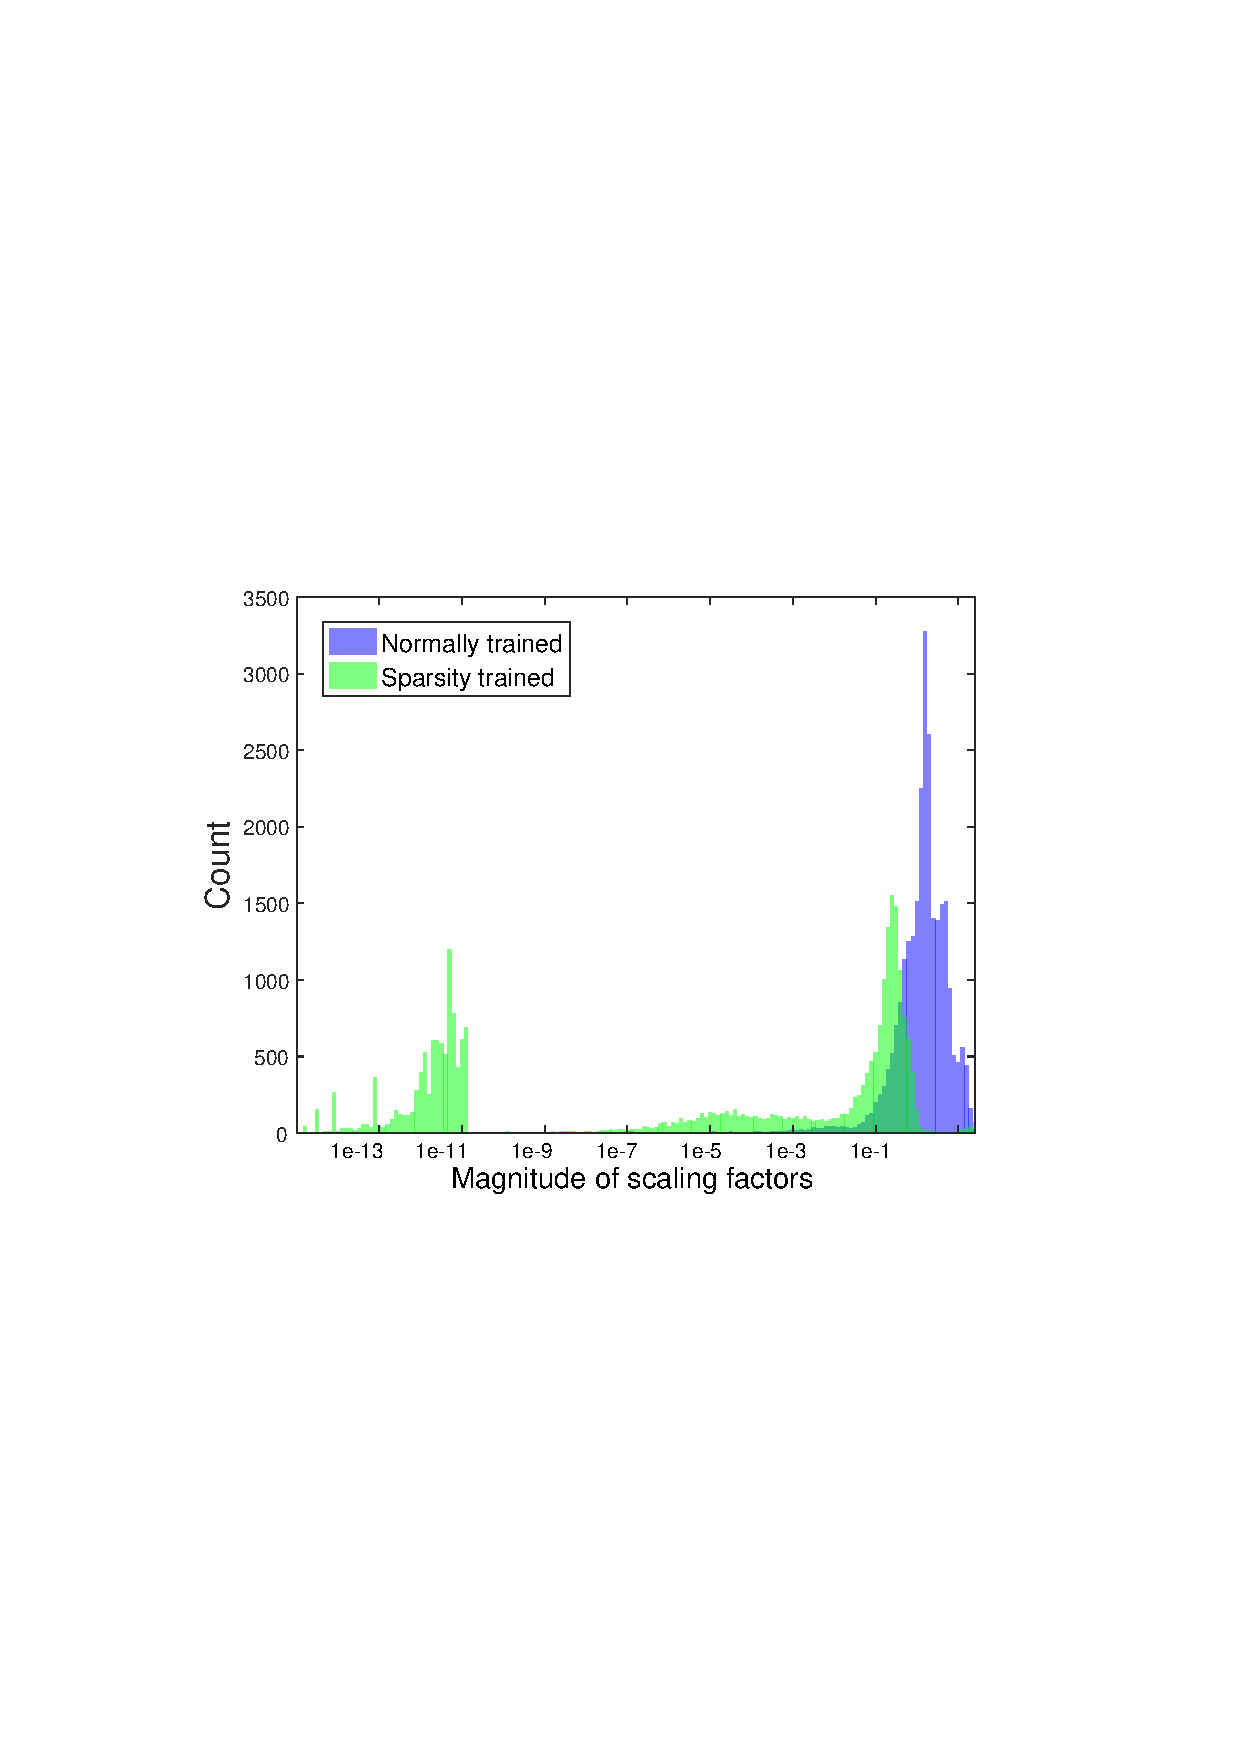
\includegraphics[width=0.5\textwidth]{figure/problem_cropped.pdf} 
 
		\caption{Distribution of scaling factors of ResNet50 before and after global sparsity training.}
		\label{pbm}
 
	\par\end{centering}

\end{figure}
 

First, from Figure \ref{pbm}, it can be seen that the right peak of the sparsely-trained network moves to 0 in some order of magnitude, compared with their location in the histogram of normally-trained network. Since the network channels corresponding to the scaling factors of this peak are preserved after the network pruning, this phenomenon indicates that the unpruned important channels are over-regularized.  We think this over-regularization prevents the better coverage of the network in the sparsity training stage, which affects the final performance of the fine-tuned pruned network.
 
Second, there are many in-between bars between the main bodies of the two peaks. This bad distribution of scaling factors challenges the threshold selecting. The channels of the in-between ares is difficult to be classified as important or not. This challenges the selecting of a optimal pruning threshold. With a sub-optimal threshold, some pruned channels may still be important for the network.

In this paper, we think the two problems are caused by the uniformly applied sparse regularization on all channels, regardless of the importance of each individual channels. Therefore, we propose a fine-grained sparsity training method which only apply the sparse regularization on the unimportant channels to keep a maximum representation ability of the important channels. 
\begin{algorithm}[t]
	\caption{Algorithm Description of MaskSparsity}
	\label{alg:FPGM}
	
	\begin{algorithmic}[1]
		\INPUT training data: $\{\mathcal{X},y\}$, pruning threshold $\theta$.
		
		\State  \textbf{Initialize}: pretrained model parameter $\mathcal{W}=\{\mathcal{W} _{i}, 0\leq i \leq L\}$;  
		
		\For{$epoch=1$; $epoch \leq epoch_{max}$; $epoch++$}
		\State Update the model parameter $\mathcal{W}$ based on $\{\mathcal{X},y\}$ and, using the global sparse regularization as in Equation~\ref{eq-tra-sp};
		\EndFor
		
		\State Obtain the pruning mask $\mathcal{M}$ by thresholding $\mathcal{W}$ with $\theta$;
		
		\State  \textbf{Reinitialize}: pretrained model parameter $\mathcal{W}=\{\mathcal{W} _{i}, 0\leq i \leq L\}$;
		
		\For{$epoch=1$; $epoch \leq epoch_{max}$; $epoch++$}
		\State Update the model parameter $\mathcal{W}$ based on $\{\mathcal{X},y\}$ , the mask-guided sparse regularization as shown in Equation~\ref{eq-Mask-sp} with the mask $\mathcal{M}$;
		\EndFor
		\State Obtain the compact model $\mathcal{W} ^{*}$ from $\mathcal{W}$;
		\State Finetune the compact model $\mathcal{W} ^{*}$;
		\OUTPUT The compact model and its parameters $\mathcal{W} ^{*}$.
	\end{algorithmic} 
\end{algorithm}
\subsection{MaskSparsity for Fine-grained Sparse Regularization}\label{MaskSP}

In this paper, we find the task of sparsity training consists of two sub-tasks implicitly. The first sub-task is identifying the unimportant channels. The second sub-task is pushing the filter weights or scaling factors of unimportant channels to 0 by the sparse regularization loss. Existing sparsity-training based methods accomplish the two sub-tasks simultaneously in the sparsity training stage. We propose to decouple the two sub-tasks. By doing this, we are able to apply the fine-grained spare regularization, which only sparse out the unimportant channels.


Figure \ref{MAskSparsityPipeline} shows the training pipeline of the proposed MaskSparsity. We transform the sparsity training stage of the existing methods into two stages. The first stage is the sparsity training stage with global sparse regularization, which is aimed to get the indexes of the unimportant channels. The indexes are transformed into a binary pruning mask in previous methods. In our method, we use the mask to identify which channels to apply the sparse regularization in the second stage. To get the pruning mask, we directly threshold the scaling factors of the normally trained network. The details is shown in Equation \ref{maskgeneration}:
\begin{equation}
	\mathcal{M} = \{\mathbbm{1}(\gamma<\theta)|\gamma \in \Gamma\},
	\label{maskgeneration}
\end{equation}
where $\mathbbm{1}$ is the indicator function, $\Gamma$ is all the scaling factors of the network, and $\theta$ is the predefined pruning threshold of the pruning method. Actually, the pruning mask $\mathcal{M}$ consists of the unimportant-channel mask of each layers, \ie $\mathcal{M} = \{ \mathcal{M}_1, \mathcal{M}_2, ..., \mathcal{M}_L \} $, where $L$ is the layer count of the network. According to Equation \ref{maskgeneration}, the pruning mask $\mathcal{M}_i$ is a binary vector consisting of 0 and 1.

As discussed above, the over-regularization on the important channels damages the network capacity. Therefore, in this paper, we design a fine-grained sparse training strategy to alleviate the damage of the sparse regularization loss on important channels.
Specifically, we propose to apply the sparse regularization only on the unimportant channels. Based on Equation \ref{eq-tra-sp}, we can describe our MaskSparsity method as the Equation \ref{eq-Mask-sp}:

\begin{equation}\label{eq-Mask-sp}
	L_{\text{Reg}}(\mathcal{I}^0, y, \mathcal{W}) = L(f(\mathcal{I}^0, \mathcal{W}), y) + \lambda \cdot  \mathcal{M} \cdot   Reg({\gamma}) \,,
\end{equation}
where $\mathcal{M}$ denote the binary mask indicating the unimportant channels of the whole network.  For the important channels, the values in the channel mask are 0. Therefore, these channels are not affected by the sparse regularization and are trained as normal. 

%\textbf{Details} 
%\subsection{ Obtaining Mask }\label{Obtaining Mask}
%Here we introduce a common way of obtaining $\mathcal{M}$. We apply the traditional sparsity-training-based method on the network in several epochs until the distribution of learn-able scaling factor converges approximately only, and prune the network base on the “smaller-norm-less-important” criterion. We can the pruning mask obtained in the pruning process as the $\mathcal{M}$ we need. The rationality of this approach is based on two points: (1) only imposing sparsity regularization on the channels that are most likely be pushed to lower orders of magnitude can minimizes the impact of penalty; (2) The convergence of the parameters distribution does not require much training epochs; (3) The sparse structure can be obtained automatically without manual experience. The MaskSparsity is summarized in Algorithm 1. 

%Due to the variety of ways of $\mathcal{M}$ acquisition, our method has a high degree of flexibility. For instance, we can obtain mask through Random search algorithm and “smaller-norm-less-important” criterion, like EagleEye[]. Geometric Median criteria[FPGM] or High-Rank criteria [HRANK] are also could be used.




\textbf{Pruning Strategy for Residual Connections. }\label{Pruning with Residual-Connections} 
Apart from solving the above two problems, the MaskSparsity method have another advantage over the other sparsity-training-based methods, which is in the case of residual connections \cite{he2016deep}. In the following, we show the pruning strategy of MaskSparsity on the structure with residual connections, and discuss its advantage. 


%We use the ResNet \cite{he2016deep} as an example to demonstrate the advantage of MaskSparsity over the other sparsity-training-based methods. 

The residual module of ResNet requires the element-wise add operation. This operation requires the summed feature maps have the same channel count. However, most of the existing pruning methods are not able to control the number of the channels that they push to zero with the sparse regularization. In this scene, they have to only prune the intersection of the unimportant channel indexes of all summed feature maps. Therefore, a number of unpruned channels are still pushed to zero by them. 
We think this increases the accuracy drop of the network pruning, because usually some of the pushed-to-zero channels still contribute to the final accuracy to some extent. The left part of Figure \ref{Pruningmask-method}(b) illustrates this problem. With MaskSparsity, the unpruned channels of these added feature maps are not sparsely regularized. Therefore, this enlarges the model capacity of the pruned network.

Moreover, in MaskSparsity, we relax the requirement of the strict intersection of the unimportant channels of all summed feature maps. For a channel index in the ResBlock \cite{he2016deep}, if it is regraded unimportant in more than $75\%$ of the summed feature maps, we set it is unimportant and apply sparsity regularization on the channels of this index in all layers of the summed feature maps. The right part of Figure \ref{Pruningmask-method} shows the unpruned channels are not sparsely regularized.
   
\begin{figure}[h!]
	\begin{centering}
		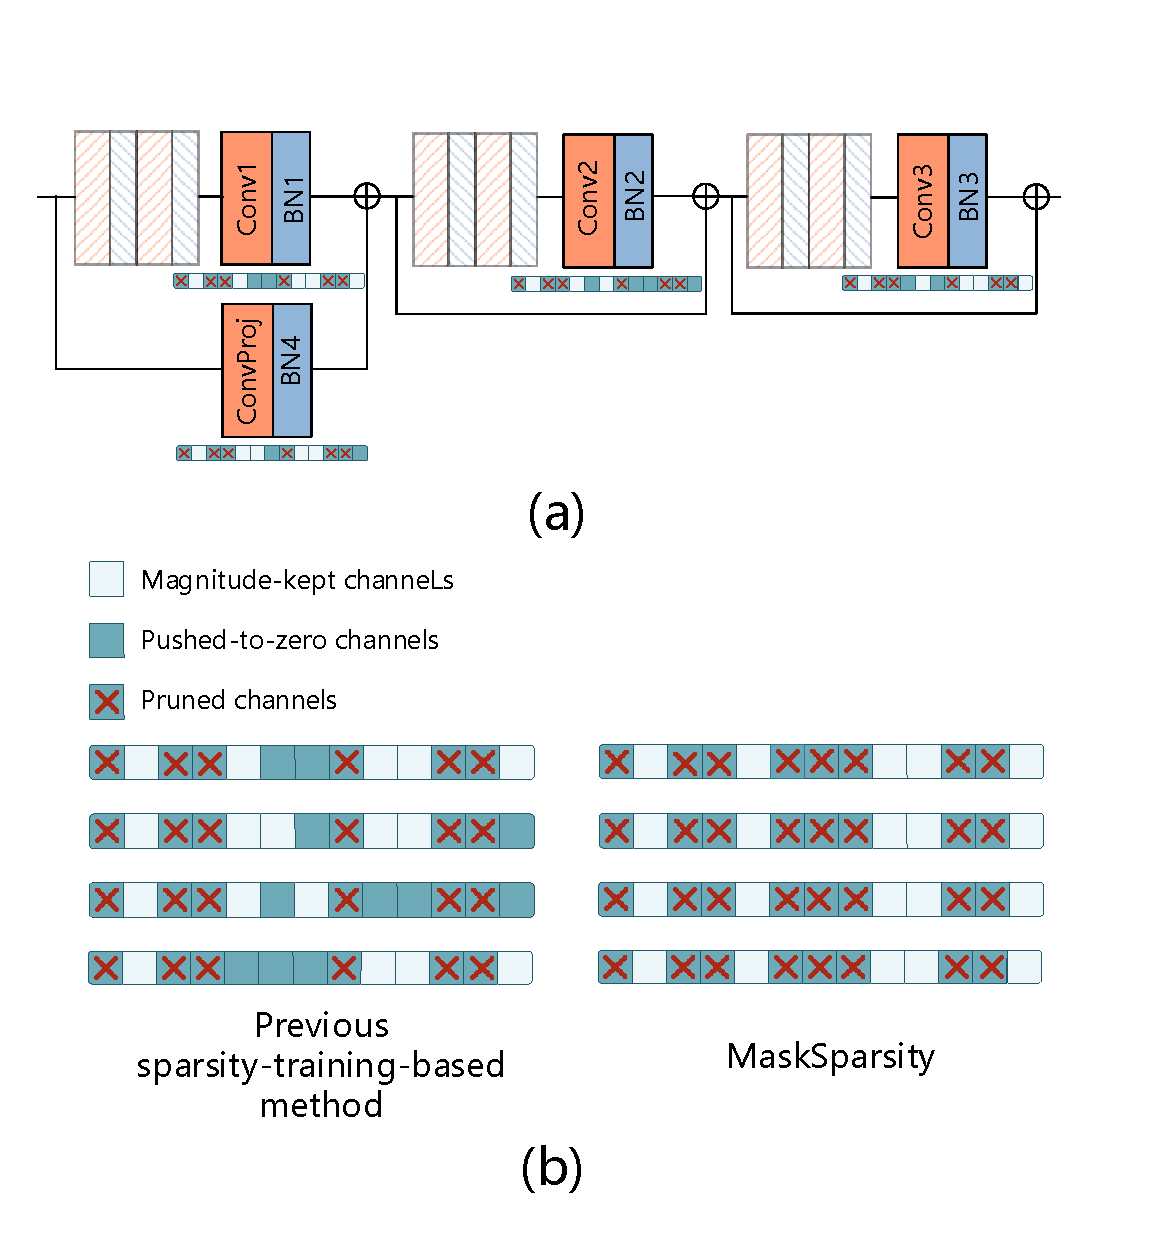
\includegraphics[width=0.5\textwidth]{figure/resduial_prune.pdf}
		\caption{
			An illustration of pruning with Residual-Connections.
			(a) shows the structure of one typical network stage. Only the last convolution layers of each ResBlock is highlighted. 
			(b) shows the pruning strategy of previous sparsity-training-based method and MaskSparsity method.
			The shallow blue boxes means the important channels.
			The deep blue boxes means the unimportant channels.
			The red cross means that the channel can be pruned.
		}
	    \label{Pruningmask-method}
	\end{centering}
    
\end{figure}

  
\begin{table*}

	\caption{Evaluation results using ResNet-50 on ILSVRC-2012.}
	\begin{center}
		\begin{small}
			
			\begin{tabular}{llccccccc}
				\toprule
				& Method 							&{Base Top-1}	&{Base Top-5}	&{Pruned Top-1}	&{Pruned Top-5}	& {Top-1 $\downarrow$ }	&	{Top-5 $\downarrow$ }	& 	{FLOPs $\downarrow$\%}	
				
				\\  \midrule  
				
				&   NS \cite{liu2017learning}          &  75.04    &    -      &   69.60   &    -      &    5.44   &  -        &   50.51   \\
				&   OT  \cite{OT}               &  75.04    &    -      &   70.40   &    -      &    4.64   &  -        &   52.88   \\
				&	SFP \cite{he2018soft}	    &	76.15 	&	92.87	&	74.61	&	92.06	&	1.54	&	0.81 	&	41.8	\\
				&GAL-0.5 \cite{GAL}				&	76.15	&	92.87	&	71.95	&	90.94	&	4.20	&	1.93	&	43.03	\\
				&HRank \cite{HRank}				&	76.15	&	92.87	&	74.98	&	92.33	&	1.17	&	0.54	&	43.76	\\
				&Hinge \cite{Hinge}             &     -     &    -      &   74.7    &    -     &     -     &       &  46.55           \\
				%&NISP \cite{yu2018nisp}			&	-		&	-		&	-		&	-		&	0.89	&	-   	&	44.01	\\	
				%&\cite{singh2018stability}		&	-		&	92.65	&	-		&	92.2	&	- 		&	0.45 	&	44.45		\\	
				%&CFP \cite{singh2018leveraging}	&	75.3	&	92.2	&	73.4	&	91.4	&	1.9 	&	0.8 	&	49.6	\\
				%&Channel Pr \cite{he2017channel}&	- 		&	92.2	&	-		&	90.8	&	- 		&	1.4 	&	50		\\
				%&SPP \cite{wang2017structured}	&	- 		&	91.2	&	-		&	90.4	&	- 		&	0.8 	&	50		\\
				&HP \cite{xu2018hybrid}			&	76.01 	&	92.93	&	74.87	&	92.43	&	1.14 	&	0.50 	&	50		\\
				%&ELR \cite{wang2018exploring}	&	- 		&	92.2	&	-		&	91.2	&	- 		&	1 		&	50		\\
				&MetaPruning \cite{Metapruning}	&	76.6	&	-		&	75.4	&	-		&	1.2		&	-		&	51.10	\\
				&Autopr \cite{luo2018autopruner}&	76.15 	&	92.87	&	74.76	&	92.15	&	1.39	&	0.72 	&	51.21	\\
				%&GDP \cite{lin2018accelerating}	&	75.13 	&	92.30	&	71.89	&	90.71	&	3.24 	&	1.59 	&	51.30	\\
				&FPGM \cite{FPGM}				&	76.15	&	92.87	&	74.83	&	92.32	&	1.32	&	0.55	&	53.5	\\
				%&SSR-L2 \cite{lin2019towards}	&	75.12 	&	92.30	&	71.47	&	90.19	&	3.65 	&	2.11 	&	55.76	\\	
				&DCP \cite{zhuang2018discrimination}&76.01 	&	92.93	&	74.95	&	92.32	&	1.06 	&	0.61 	&	55.76	\\		
				%&C-SGD \cite{CSGD}				&	75.33	&	92.56	&	74.54	&	92.09	&	0.79 	&	0.47 	&	55.76	\\
				&ThiNet \cite{DBLP:journals/pami/LuoZZXWL19}&	75.30	&	92.20	&	72.03	&	90.99	&	3.27 	&	1.21 	&	55.83	\\
				%&SASL \cite{SASL}				&	76.15	&	92.87	&	75.15	&	92.47	&	1.00	&	0.40	&	56.10	\\
				&\textbf{MaskSparsity (ours)}	&	\textbf{76.44}	&	\textbf{93.22}	&	\textbf{75.50}	&	\textbf{92.72}	&	\textbf{0.93}	&	\textbf{0.49}	&	53.761	\\
				%&TRP \cite{TRP}					&	75.90	&	92.70	&	72.69	&	91.41	&	3.21	&	1.29	&	56.52	\\
				%&LFPC \cite{he2020learning}		&	76.15	&	92.87	&	74.46	&	92.32	&	1.69	&	0.55	&	60.8	\\
				
				%&DMC \cite{}				&	76.15	&	92.87	&	-	&	-	&	0.8	&	0.38	&	55.0	\\
				
				
				
				&HRank \cite{HRank}				&	76.15	&	92.87	&	71.98	&	91.01	&	4.17	&	1.86	&	62.10	\\
				%&GAL-1-joint					&	76.15	&	92.87	&	69.31	&	89.12	&	x		&	x		&	72.86	\\
				%&EagleEye \cite{}					&	-	&	-		&	76.4	&	92.89		&	-		&	-		&	50	\\
			%	&HRank	\cite{HRank}							&	76.15	&	92.87	&	69.10	&	89.58	&	7.05	&	3.29	&	76.03	\\
				\bottomrule
				
			\end{tabular}
		\end{small}
	\end{center}
	\vspace{-0.1in}
	\label{exp-table-imgnet}
\end{table*}
\section{Experiments}\label{Experiment}
\subsection{Experimental Settings}

\textbf{Datasets and Baselines}.
To demonstrate the effectiveness of Mask Sparsity in reducing model complexity, we evaluate MaskSparsity on both small and large datasets,  \emph{i.e.}, CIFAR-10 \cite{krizhevsky2009learning} ,and ILSVRC-2012 \cite{russakovsky2015imagenet}. The CIFAR-10 dataset consists of natural images of 10 classes with resolution 32$\times$32 and the train and test sets contain 50,000 and 10,000 images respectively. The ImageNet dataset consists of natural images of 1000 classes with resolution 224$\times$224 and the train and test sets contain 1.2 million and 50,000 images respectively.  We experiment with ResNet-50 \cite{He2016IdentityMI} on ILSVRC-2012 , and experiment with ResNet-56 \cite{he2016deep} and ResNet-110 \cite{he2016deep} on CIFAR-10.

\textbf{Evaluation Protocols}.
For fair comparison of the model complexity, we use the number of parameters and the FLOPS \cite{he2016deep}. To evaluate the accuracy, to be consistent with other methods, we use top-1 and top-5 score of full-size models and pruned models on ILSVRC-2012 and top-1 score only on CIFAR-10.

\textbf{Training and Pruning setting}.


On CIFAR-10, we train models for 200 epochs with a batch size of 128, a weight decay of 0.0005, a Nesterov momentum of 0.9 without dampening in every stage, and an initial learning rate of 0.1 which is divided by 5 at epochs 60, 120 and 160 on four NVIDIA GTX 1080Ti GPUs; On ILSVRC-2012, we train models for 100 epochs with a batch size of 256, a weight decay of 0.0001, a Nesterov momentum of 0.9 with dampening in every stage, and an initial learning rate of 0.1 which is divided by 5 at epochs 30, 60 and 90 on eight NVIDIA GTX 1080Ti GPUs.

In the mask acquisition step, we first perform sparsity training on resnet56 with penalty factors $\lambda=2e^{-4}$, resnet110 with penalty factors $\lambda=5e^{-5}$ on CIFAR-10, and resnet50 with penalty factors $\lambda=2e^{-4}$ on ILSVRC-2012. Then we prune the sparse model base on the “smaller-norm-less-important” criterion and obtain the sparse mask according to the target pruning rate. 

In the mask sparsity training step, we reinitialize the network with a pretrained model and perform the mask sparsity training for the model with pruning the mask and a higher $\lambda$. On CIFAR-10, we choose $\lambda=1e^{-3}$ for ResNet-56 and ResNet-110, and we choose $\lambda=5e^{-4}$ for ResNet-50 On ILSVRC-2012. 

In the formal pruning stage, we prune the model with a threshold of $1e^{-2}$. The pruning mask and sparse mask almost completely coincide,  which means that we only perform a sparse penalty on the pruned channel.

After pruning, we fine-tune the pruned model with an initial learning rate of 0.001, and
other parameter settings are the same as the previous step.


%--------------------------------------------------------------------------------------------------------------------------------------------------

\subsection{Results and Analysis}

\subsubsection{Results on ILSVRC-2012}\label{results_on_ILSVRC-2012}
As shown in Table \ref{exp-table-imgnet}, our proposed MaskSparsity achieves the new state-of-the-art. NS \cite{liu2017learning} is the baseline method of MaskSparsity, which adopt the global sparse regularization on the scaling factors of BN layers. OT \cite{OT} is the improved NS method, which set an optimal threshold for each layer. It can be seen that the MaskSparsity outperforms them significantly in the respect of accuracy drop (Top-1 $\downarrow$  and Top-5 $\downarrow$  in Table \ref{exp-table-imgnet}) under roughly the same level of FLOPS drop. This shows that with the fine-grained sparse regularization, we avoid the bad effect of the sparse regularization on the unpruned channels. Moreover, as shown in Section \ref{abalation}, with MaskSparsity, the pruning threshold on the scaling factors is easier to set.

In Table \ref{exp-table-imgnet}, it can be seen that we also outperform the non-sparsity-training-based methods under the same FLOPS decrease rate, \eg, FPGM \cite{FPGM} (53.5\% FLOPS reduced), and DCP \cite{zhuang2018discrimination} (55.76\% FLOPS reduced), MetaPruning \cite{Metapruning} (51.10\% FLOPS reduced). While the FLOPS reduction of MaskSparsity is less than HRank (53.76\% vs 62.1\%), the accuracy of the pruned model is much higher than that of HRank (0.93 vs 4.17 in Top-1 accuracy drop).
This shows that GroupSparsity's superiority over the previous state-of-the-art methods.
 
%Under similar FLOPs with Network Slimming \cite{liu2017learning} and Optimal Thresholding \cite{OT}, MaskSparsity achieves only $1\%$ top-1 accuracy drop with ResNet-56, while Network Slimming achieves $5.44\%$ top-1 accuracy drop and Optimal Thresholding achieves $4.64\%$ top-1 accuracy drop.
 
%Moreover, compared with traditional non-sparsity-training-based methods, our method is also slightly improved. HRank reduces $43.76\%$ FLOPS with $1.17\%$ top-1 accuracy drop, but MaskSparsity achieves $53.76\%$ Flops reduction with $1.03\%$ top-1 accuracy drop. Comparing to FPGM, when  pruning $53\%$ FLOPs of ResNet-50, our accuracy drop ($1.03\%$) is much less then FPGM ($1.32\%$). 

\subsubsection{Results on CIFAR-10}\label{results_on_cifar10}

Table \ref{exp-table-cifar10-r56} shows the experimental results of ResNet-56 on CIFAR-10. On this small dataset, MaskSparsity also achieves the state-of-the-art performance. Under similar FLOPs reduction with FPGM \cite{FPGM} and Hinge \cite{Hinge}, MaskSparsity achieves $0.31\%$ Top-1 accuracy drop with ResNet-56, which is slightly better than FPGM \cite{FPGM} (0.31\% vs 0.33\%) and Hinge \cite{Hinge} (0.31\% vs 0.74\%).

Table \ref{exp-table-cifar10-r110} shows the experimental results of another network, ResNet-110 on CIFAR-10. With this deeper network, MaskSparity achieves a better performance. As shown in Table \ref{exp-table-cifar10-r110}, our MaskSparsity outperforms the other state-of-the-art methods, like HRank \cite{HRank} (at 58.2\% FLOPS reduction), under the roughly the same ratio of FLOPS reduction. MaskSparsity has roughly the same accuracy increase with FPGM \cite{FPGM} and C-SGD \cite{CSGD} (0.02 vs 0.06 and 0.03), but MaskSparsity has a larger FLOPS reduction than these two methods(63.03\% vs 52.3\% and 60.89\%).
  







%--------------------------------------------------------------------------------------------------------------------------------------------------

%--------------------------------------------------------------------------------------------------------------------------------------------------
\begin{table}[ht]\small
	\caption{Evaluation results using ResNet-56 on CIFAR-10.}

	\setlength{\tabcolsep}{0.01em}
	\begin{center}
		\begin{tabular}{ccccc}	
			\hline
			
			Method 							&Base top-1		&Pruned top-1	& Top-1 $\downarrow$\% 	&FLOPs$\downarrow$\%	 			\\
 			 \hline
			
			%Li et al. \cite{li2016pruning}					&	93.04	&	93.06			&	-0.02 	&	27.60	\\
			%NISP-56 \cite{yu2018nisp}				&	-		&	-				&	0.03 	&	43.61	\\
			%Zhu et al. \cite{zhu2018improving}					&	93.39	&	93.40			&	-0.01 	&	47.36	\\
			%L1 \cite{li2017pruning}    &93.26                            &93.06              &0.2   &14.1\% \\
			%
		
			%NISP \cite{yu2018nisp}   &93.26         &93.01   &0.025            &35.5\%       \\
			%
			
			%
		    NISP \cite{yu2018nisp}   &-         &-   &0.03 &42.6 \\
			
            Hinge \cite{Hinge}   &93.69        &92.95   &0.74            &50       \\
			Channel Pruning \cite{he2017channel}	&	92.8	&	91.8			&	1.0 	&	50		\\
			AMC \cite{he2018amc}					&	92.8	&	91.9			&	0.9		&	50		\\
			%HRank \cite{HRank}						&	93.26	&	93.17			&	0.09	&	50.0	\\
			He \emph{et al}. \cite{he2017channel}    &93.26      &90.80   &2.46             &50.6       \\
			
			LeGR \cite{LeGR}   &93.9        &93.7   &0.2            &52 \\
			
			
			FPGM \cite{FPGM}						&	93.59	&93.26	&	0.33	&	52.6\\
			%SFP \cite{he2018soft}					&	93.59	&93.35	&	0.24	&	52.6\\
			LFPC \cite{he2020learning}				&	93.59	&93.24	&	0.35	&	52.9\\
			\textbf{MaskSparsity (ours)}			&	\textbf{94.50}	&	\textbf{94.19}	&\textbf{0.31}	& 54.88	\\	
			%SASL \cite{SASL}						&	93.63	&	93.58			&	0.05	&	57.1	\\
			GAL-0.8 \cite{GAL}   &93.26      &90.36     &2.9         &60.2  \\
			
			%GAL-0.8									&	93.26	&	91.58			&	1.68	&	60.2	\\
			%AFP \cite{ding2018auto}					&	93.93	&	92.94			&	0.99 	&	60.85	\\
			%C-SGD \cite{CSGD}						&	93.39	&	93.62			&	-0.23 	&	60.85	\\
			HRank \cite{HRank}		&	93.26	&	90.72			&	2.54	&	74.1	\\
			%ResRep (ours)							&	93.71	&	92.94			&	0.67	&	75.12	\\
			%TRP \cite{TRP}							&	93.14	&	91.62			&	1.52	&	77.82	\\
			 
			\hline
			
		\end{tabular}
	\end{center}
	\label{exp-table-cifar10-r56}
\end{table}
%--------------------------------------------------------------------------------------------------------------------------------------------------

%--------------------------------------------------------------------------------------------------------------------------------------------------
\begin{table}[ht]
	\caption{Evaluation results using ResNet-110 on CIFAR-10.}
	\vspace{-0.4cm}
	\small
	\setlength{\tabcolsep}{0.01em}
	\begin{center}
		\begin{tabular}{ccccc}
			\hline
			
			Method 							&Base top-1		&Pruned top-1	& Top-1 $\downarrow$\% 	&FLOPs$\downarrow$\%	 			\\
			\hline
			
			
			Li et al. \cite{li2016pruning}		    &	93.53	&	93.30	&	0.23 		&	38.60	    \\
			SFP \cite{he2018soft}					&	93.68	&	93.86	&	-0.18	    &	40.8	    \\
			NISP-110 \cite{yu2018nisp}				&	-		&	-		&	0.18		&	43.78		\\
			GAL-0.5 \cite{GAL}						&	93.50	&	92.74	&	0.76		&	48.5		\\
			
			FPGM \cite{FPGM}		&93.68	&93.74	&	-0.06	&	52.3\\

			
			
			HRank \cite{HRank}						&	93.50	&	93.36	&	0.14		&	58.2		\\
			
			LFPC \cite{he2020learning}				&	93.68	&	93.07	&	0.61	    &	60.3	    \\
			%C-SGD \cite{CSGD}						&	94.38	&	94.41	&	-0.03		&	60.89		\\
			\textbf{MaskSparsity (ours)}	&	\textbf{94.70}	&	\textbf{94.72}	&	\textbf{-0.02}	&	\textbf{63.03}\\
			HRank \cite{HRank}		&	93.50	&	92.65	&      0.85		&	68.6		\\
		
		
		   	C-SGD \cite{CSGD}						&	94.38	&	94.41	&	-0.03		&	60.89		\\
		    HRank									&	93.50	&	92.65	&	0.85		&	68.6		\\
		    
		    SASL \cite{SASL}						&	93.83	&	93.80	&	0.03		&	70.2		\\
		 
			
			\hline
			
		\end{tabular}
	\end{center}
	\label{exp-table-cifar10-r110}
\end{table}
%--------------------------------------------------------------------------------------------------------------------------------------------------
 



\begin{table}[ht]
	\caption{Pruning VGG16 on CIFAR-10.}
	\vspace{+0.2em}
	%\small
	\scriptsize
	\setlength{\tabcolsep}{0.35em}
	\begin{center}
		\begin{tabular}{cccccc}
			\hline
			
		Method 			&Basetop-1		&\shortstack {Pruned\\before FT} &Fine-tuned	& Top-1 $\downarrow$\% 	&FLOPs$\downarrow$\% \\ 
		\hline
		
		PFEC~\cite{li2016pruning} {\scriptsize{( from \cite{FPGM})}}   & 93.58  &77.45 & 93.28 & 0.3  &34.2\\  
		
		FPGM \cite{FPGM}   & 93.58  &80.38 & 94.00  &\textbf{-0.42} &34.2\\  
		
		NS \cite{liu2017learning} & 93.66 &-  & 93.80  &-0.14 &51\\  
		
    	\textbf{MaskSparity(ours)}                &\textbf{93.86}   &\textbf{94.16} &\textbf{94.24} &-0.38 & \textbf{52.21}\\ 
			
		
		    
			\hline
		
		\end{tabular}
	\end{center}
	\label{exp-table-cifar10-VGG16}
\end{table}
%--------------------------------------------------------------------------------------------------------------------------------------------------








\subsection{Ablation Study}\label{abalation}
\textbf{Visualization of the distribution of the scaling factors after using MaskSparsity.} 
In Section \ref{Analysisoftraditionalsp} and Figure \ref{pbm}, we show that the distribution of scaling factors meets two problems that might harm the pruning performance. In Figure \ref{dstbtion-mask-sp} we draw the same set of scaling factors after the mask-guided sparse regularization, and compare it with that of the pre-trained networks. It can be seen that the two problems are alleviated significantly. First, the right peak of the sparsity trained network does not move towards the 0 like in Figure \ref{pbm}. Second, the two peaks are well distinguishable, with almost no in-between bars in the middle area. This demonstrates the effectiveness of the fine-grained sparse regularization of MaskSparsity, which would benefit the pruning performance.
  

\textbf{The convergence analysis by visualizing the gradients.} To validate the statement that the sparse regularization on unpruned channels restricts the network's capacity, we visualize the gradients of important and unimportant channels after the sparsity training using global and fine-grained sparse regularization, respectively. The result is shown in Figure \ref{grad}. The gradients are collected by continue training for 1,000 iterations from the end of the sparsity training stage of ResNet-50 on ILSVRC-2012. In Figure \ref{grad} (a), it can be seen that the gradient norm of the important channels is still large for the important channels with the global sparse regularization, while Figure \ref{grad} (b) shows the important channel has a small gradient norm with our fine-grained MaskSparsity sparse regularization. Figure \ref{grad} (b) and (d) shows that both the gradients of unimportant channels with the two kind of sparse regularization methods are almost the same. According to these figures, the global sparse regularization leads to a larger gradient on the important channels though the network's accuracy and sparsity have converged. We infer the large gradient prevent the network converge to a better local-minimum.

\textbf{The effectiveness of fine-grained sparse regularization on residual modules.} In Section \ref{MaskSP} and Figure \ref{Pruningmask-method}, we claim that the MaskSparsity avoids to apply sparse regularization on the unpruned unimportant channels, which can make the network make full use of all kept channels to maximum its accuracy. In Figure \ref{Pruning-mask-exp}, we plot the binary unimportant-channel masks of each layer of the third stage of ResNet-56, which are generated by thresholding the scaling factors. It can be seen that the binary masks of MaskSparsity is much consistent among the channels of the same channel index. This shows the benefit of the fine-grained sparsity from MaskSparsity.

\textbf{The robustness to various pruning thresholds.} 


\textbf{Comparing fine-tuning and train-from-scratch.} 
In Table \ref{Finetune_scratch_cifar10}, we list the network model's accuracy and computational complexity at different pruning stages. Moreover, we also list the result that train the pruned model from scratch without exploiting its weights. It can be seen that the train-from-scratch result is lower than the fine-tuning result. We think this demonstrates the effectiveness of the fine-grained sparsely-trained pre-trained weights.


 \begin{figure}[h!]
\begin{centering}
	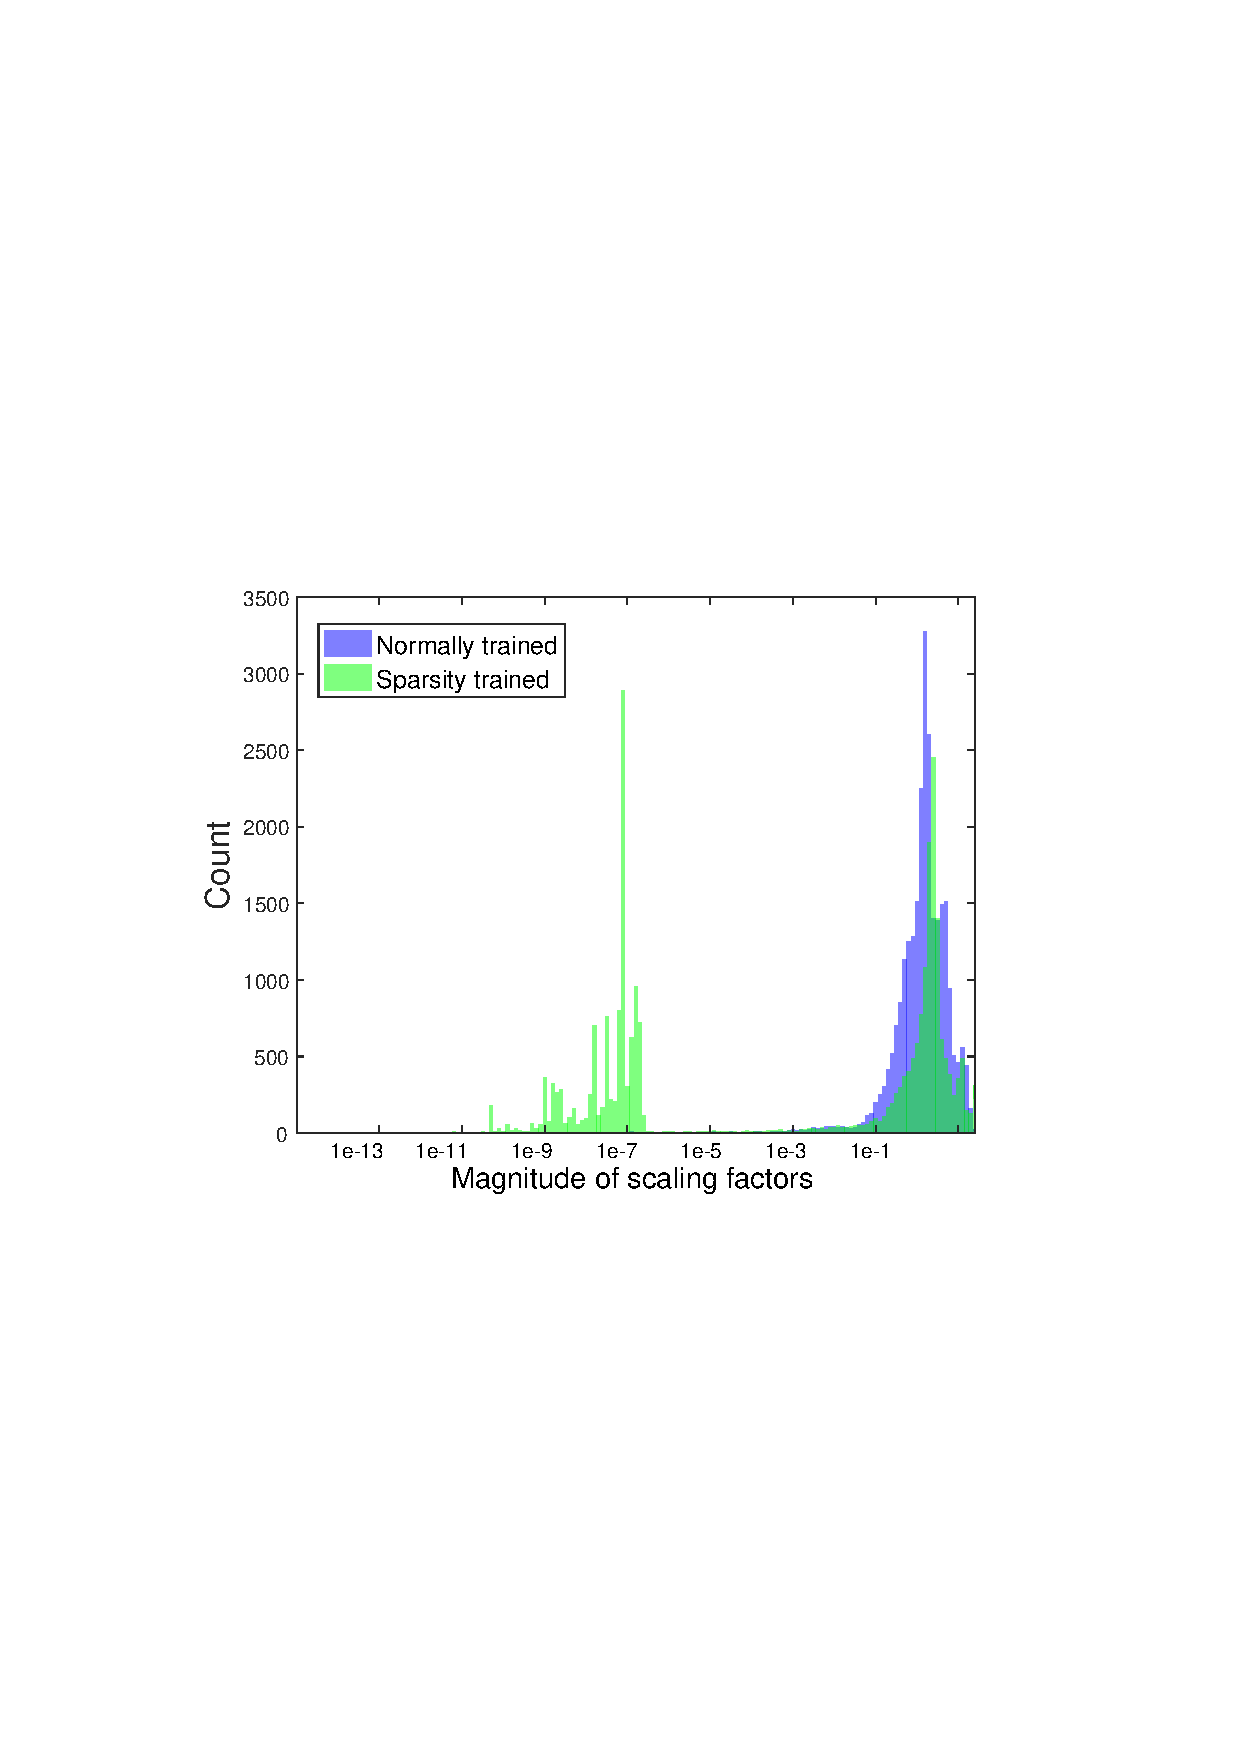
\includegraphics[width=0.5\textwidth]{figure/solve_pbm_cropped.pdf} 
	\caption{Distribution of scaling factors of ResNet50 on ILSVRC-2012 before and after the MaskSparsity's sparsity training.}
	\label{dstbtion-mask-sp}
	\par\end{centering}
\end{figure}

\begin{figure}[h!]
	\begin{centering}
		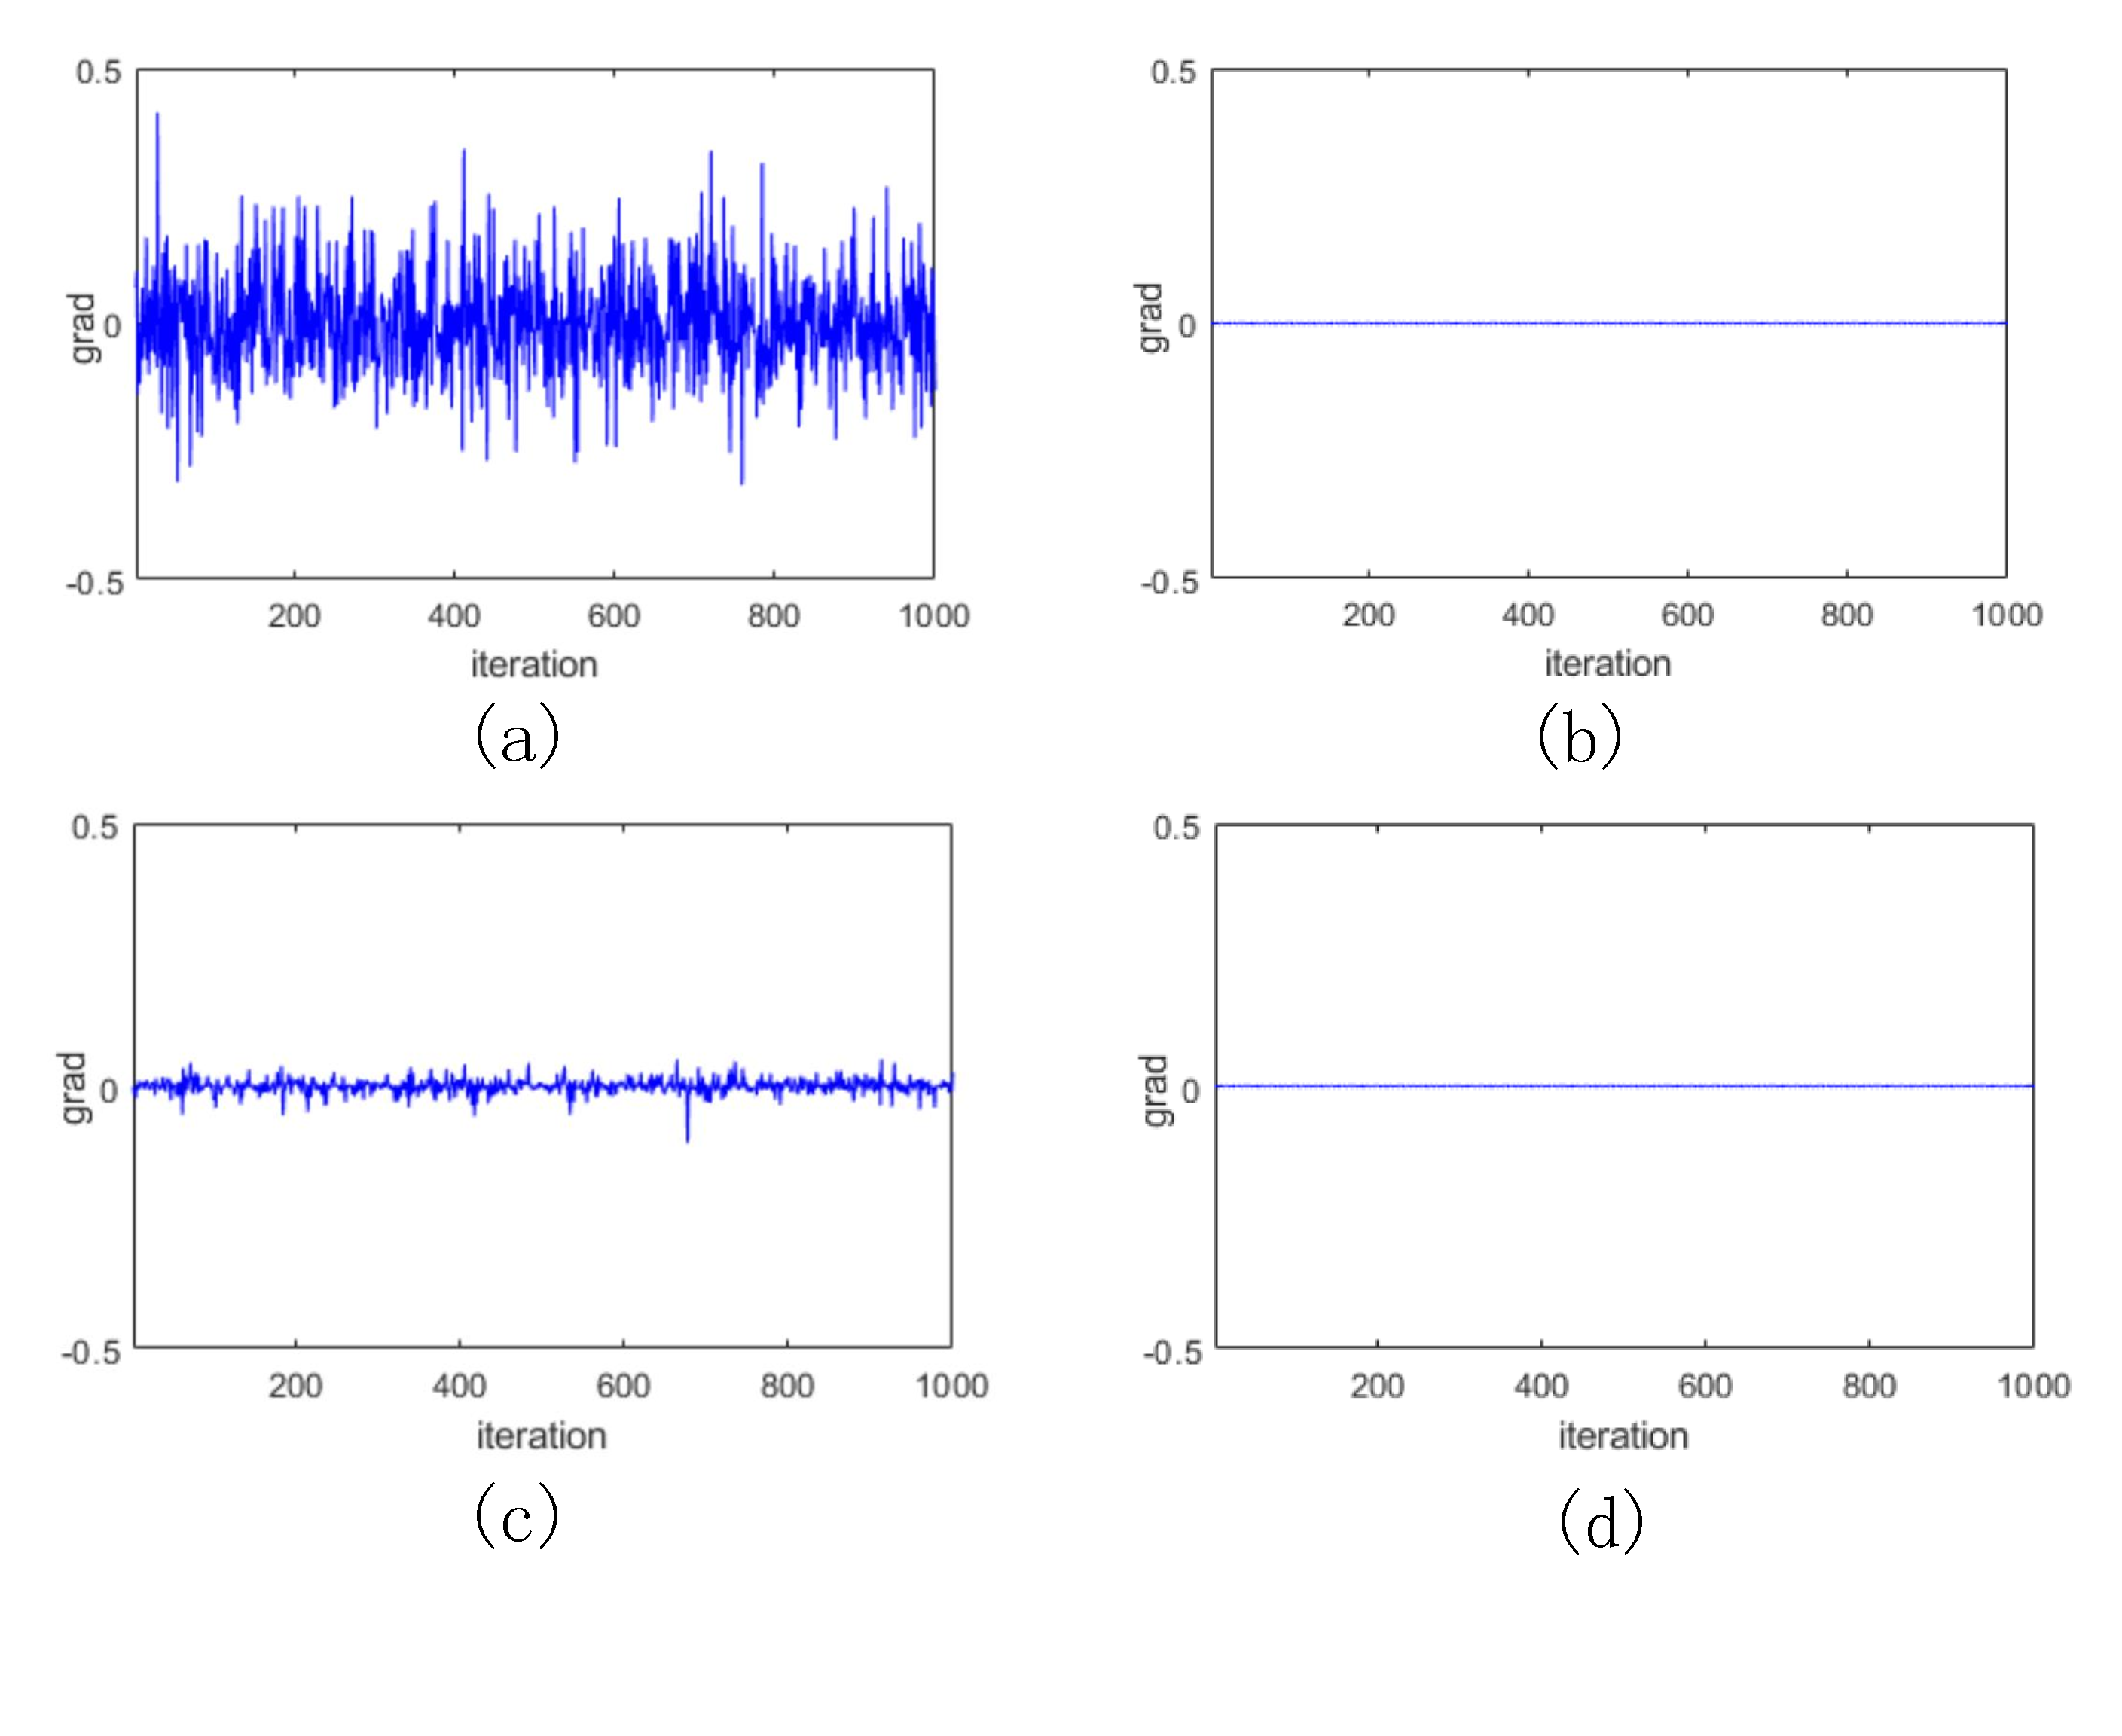
\includegraphics[width=0.5\textwidth]{figure/grad2_cropped.pdf}
		\caption{The gradients of the scaling factors of a certain channel over the additional 1, 000 sparsity-training iterations after the ending of the sparsity training stage. The spare regularization keep the same as that used in the original sparsity training. We choose an important channel and an unimportant channel to conduct this experiment. (a) The important channel, global sparse regularization. (b) The unimportant channel, global sparse regularization. (c) The important channel, fine-grained sparse regularization of MaskSparsity. (d) The unimportant channel, fine-grained sparse regularization of MaskSparsity.}
		\label{grad}
		\par\end{centering}
\end{figure}

 
\begin{figure}[h!]
	\begin{centering}
		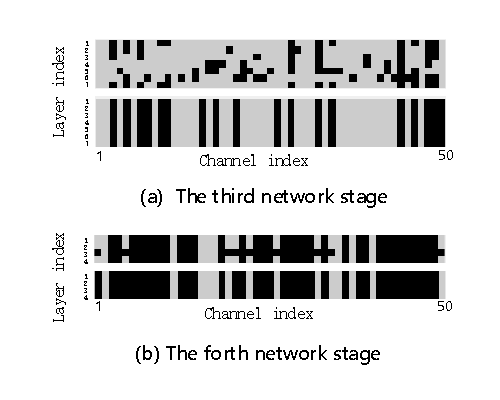
\includegraphics[width=0.5\textwidth]{figure/stage_mask_ablationstudy.pdf} 
	    \caption{ The unimportant-channel masks in every last layers of ResBlocks in the third and forth network stage.	The data were obtained from ResNet50 trained with traditional sparsity-training-based methods and MaskSparsity on ILSVRC-2012.
    	}
        \label{Pruning-mask-exp}
    \par\end{centering}
\end{figure}

  %we show the pruning mask fragments of resnet-56's four stages  obtained by  traditional sparsity-training-based methods and MaskSParsity respectively on ILSVRC-2012.  It needs to be explained here that some channels are selected to sparse but not be pushed below the pruning threshold, because L1 cannot sparse all the selected channels to be near zero ;some channels without sparsity constraint are reduced to zero, because weight decay and ReLU operation can also cause sparsity [On Implicit Filter Level Sparsity in Convolutional Neural Networks],But despite this, the experimental results still prove the effectiveness of the method.

 
  

\begin{table}[ht]

	\caption{The stage-wise performance in the case of  pruning ResNet-56 on CIFAR-10.}
	\small
	\setlength{\tabcolsep}{0.5em}
	\begin{center}
		\begin{tabular}{lllll}
			\toprule
		&Model state               &Top-1\%           &FLOPs          &Parameters \\
		\midrule
		&Normally trained      &94.50            &126M      &853K  \\
		%
		&MaskSparsity trained        &94.02             &126M      &853K  \\
		%
		
		&Pruned      &92.67             &57M     &419K  \\
		%
		&Finetune       &94.19             &57M    &419K \\
		%
		\hline
		&Train from Scratch   &93.60            &57M  &419K  \\
		%
		\bottomrule
			
		\end{tabular}
	\end{center} 
	\label{Finetune_scratch_cifar10}
\end{table}


 
\begin{table}[ht]

	\caption{Pruning ResNet56 on CIFAR-10.}
	\small
	\setlength{\tabcolsep}{0.5em}
	\begin{center}
		\begin{tabular}{lllll}
			\toprule
			Pruning threshold               &Top-1\%           &FLOPs          &Parameters \\
			\midrule
			Before pruning & 94.02      &126M      &853K  \\
			$1e^{-1}$     & 85.63      &54M      &408K  \\
			%
		    $1e^{-2}$     & 92.67      &57M      &419K  \\
		    %
		    $1e^{-3}$     & 92.56      &57M      &419K  \\
		    %
		    $1e^{-4}$     & 92.59      &57M      &421K  \\
		    %
		    $1e^{-5}$     & 93.01      &58M      &422K  \\
		    %
		    $1e^{-6}$     & 94.02      &90M      &620K  \\
		    %
			\bottomrule
			
		\end{tabular}
	\end{center} 
	\label{pruning_threshold}
\end{table}
 






In order to make a fair comparison and remove the influence of insufficient convergence, we use the same parameter configuration as normal train, except for the base learning rate, and enough epochs for scratch training and fine-tune. As show in Tab \ref{Finetune_scratch_cifar10}. The results show that fine-tune result is nearly  $1\%$ top-1 accuracy  higher than training from scratch.
 


\section{Conclusion}\label{Conclusion}

In this paper, to solve the problem that existing sparsity-training-based methods over-regularize the important channels, we design a network pruning method with the fine-grained sparse regularization, named MaskSparsity. MaskSparsity apply the sparse regularization only on the unimportant channels which are to be pruned. Therefore, MaskSparsity can minimize the negative impact of the sparse regularization on the important channels. The method is effective and efficient, without too many hyper-parameter settings. The experimental results show that it outperforms the other sparsity-training-based pruning methods and achieves the state-of-the-art on the benchmarks. In the future, we plan to work on how to obtain better pruning masks.


{\small
\bibliographystyle{ieee_fullname}
\bibliography{egbib}
}

\end{document}
